% -*- root: ../main.tex -*-

% Esporre i principali problemi affrontati durante l'effettiva realizzazione delle componenti hardware/software e illustrare le soluzioni implementative adottate. Se l'elaborato ha previsto l'utilizzo di tecnologie già disponibili sul mercato, discuterne brevemente le caratteristiche e motivarne l'adozione rispetto ad altre soluzioni assimilabili. NOTA: in questa sezione devono essere riportate esclusivamente le porzioni di codice ritenute particolarmente significative.

\chapter{Implementazione}
\section{Server}
\textit{Commento: questo secondo me è da fare insieme, ognuno può aggiungere qualcosa della propria parte. Magari scrive uno e l'altro se vuol dire qualcosa anche della sua parte la aggiunge.}

Per la parte backend ci si è avvalsi della tecnologia Nodejs + Express + MongoDb per il database.\\
Per l'invio delle email gestito nel backend è stato utilizzato un modulo di NodeJs chiamato Nodemailer.\\
Inoltre ci si è avvalsi della libreria Sockets.Io per una comunicazione bidirezionale tra client e server.

Si riportano ora alcuni aspetti implementativi del server che si ritiene opportuno evidenziare. 
\subsection{Forecast e Socket.IO}
scrivi se c'è qualche capitolo interessante da dire

\subsection{Autenticazione}

\subsubsection{JSON Web Token JWT}
Per l'autenticazione è stato deciso di utilizzare il sistema a token JWT, firmati dal backend. Al momento
del login il server rilascia un token al client contenente dei dati
utili all’autenticazione; in questa maniera, durante le successive richieste,
il client invierà anche il token ricevuto, e il server lo controllerà per verificare
se è valido e quindi autorizzare il client. In questa maniera il server
diventa stateless, non avendo bisogno di salvare le informazioni relative
alle sessioni dei vari client collegati.


\begin{lstlisting}[language=Javascript]
// generate token when user log in
userSchema.methods.generateToken = function (cb) {
  var user = this;
  var token = jwt.sign({ _id: user._id }, process.env.SECRET);
  user.token = token;
  user.save(function (err, user) {
    if (err) return cb(err);
    cb(null, user);
  });
};
// find by token
userSchema.statics.findByToken = function (token, cb) {
  var user = this;
  jwt.verify(token, process.env.SECRET, function (err, decode) {
    user.findOne({ _id: decode, token: token }, function (err, user) {
      if (err) return cb(err);
      cb(null, user);
    });
  });
};
//delete token, when the user logout
userSchema.methods.deleteToken = function (token, cb) {
  var user = this;

  user.update({ $unset: { token: 1 } }, function (err, user) {
    if (err) return cb(err);
    cb(null, user);
  });
};

\end{lstlisting}

Per facilitare l'utilizzo della validazione del token JWT è stato prodotto un middleware facilmente inseribile nel 
usso di Express. Questo middleware recupera il token disponibile dai cookies, inoltre recupera i dati sull'utente
autenticato e li inserisce nella richiesta per renderli disponibili nel handler della
route desiderata.
\begin{lstlisting}[language=Javascript]
let auth = (req, res, next) => {
  let token = req.cookies.auth;
  if (!token) {
    // Response the missing token result.
    return res.status(401).json({
      error: "Missing auth token in the request.",
    });
  }

  User.findByToken(token, (err, user) => {
    if (err) throw err;
    if (!user)
      // Notify the unauthorized access.
      return res.status(403).json({
        error: "Didn't found any user matching the auth token provided.",
      });

    // Use the found data in next handler.
    req.token = token;
    req.user = user;
    next();
  });
};

\end{lstlisting}
\subsubsection{Dati sensibili}
Si è avuta la necessità anche di gestire alcuni dati sensibili dell'utente, come le password. E' stata utilizzata bcrypt, una funzione di hashing per salvare le password in maniera sicura
nel database; viene utilizzato al momento della registrazione di un utente
quando si deve salvare la password nel db (viene salvato il suo hash con il
relativo valore di sale), e al login quando bisogna confrontare la password
ricevuta dall’utente con quella salvata. 
\begin{lstlisting}[language=Javascript]
userSchema.pre("save", function (next) {
  var user = this;
  if (user.isModified("password")) {
    bcrypt.genSalt(salt, function (err, salt) {
      if (err) return next(err);
      bcrypt.hash(user.password, salt, function (err, hash) {
        if (err) return next(err);
        user.password = hash;
        next();
      });
    });
  } else {
    next();
  }
});
userSchema.methods.comparePassword = function (password, cb) {
/*Comparing the user password when user tries to login*/
  bcrypt.compare(password, this.password, function (err, isMatch) {
    if (err) return cb(next);
    cb(null, isMatch);
  });
};
\end{lstlisting}

\subsection{Prossimo sottocapitolo ...}


\section{Client}
\textit{Commento:anche questo da completare come nel server, ci ho messo qualche spunto}\\
Per lo sviluppo del Client è stato usato Vuetify, un framework di componenti di Material Design per Vue. js che consente agli sviluppatori di creare incredibili applicazioni in modo rapido ed efficiente.
Si riportano ora alcuni aspetti implementativi del server che si ritiene oppurtuno evidenziare: 
\subsection{Socket}
TODO

\subsection{Store}
Come tutte le applicazioni Vuex c'è uno store che è un po' un singleton, che contiene tutti i dati in un oggetto.
Graficamente potremo delinearne così la struttura:
\begin{figure}[H]
    \caption{Le azioni sono fuori dallo store e diventano servizi}
    \label{fig:Store}
    \centering
    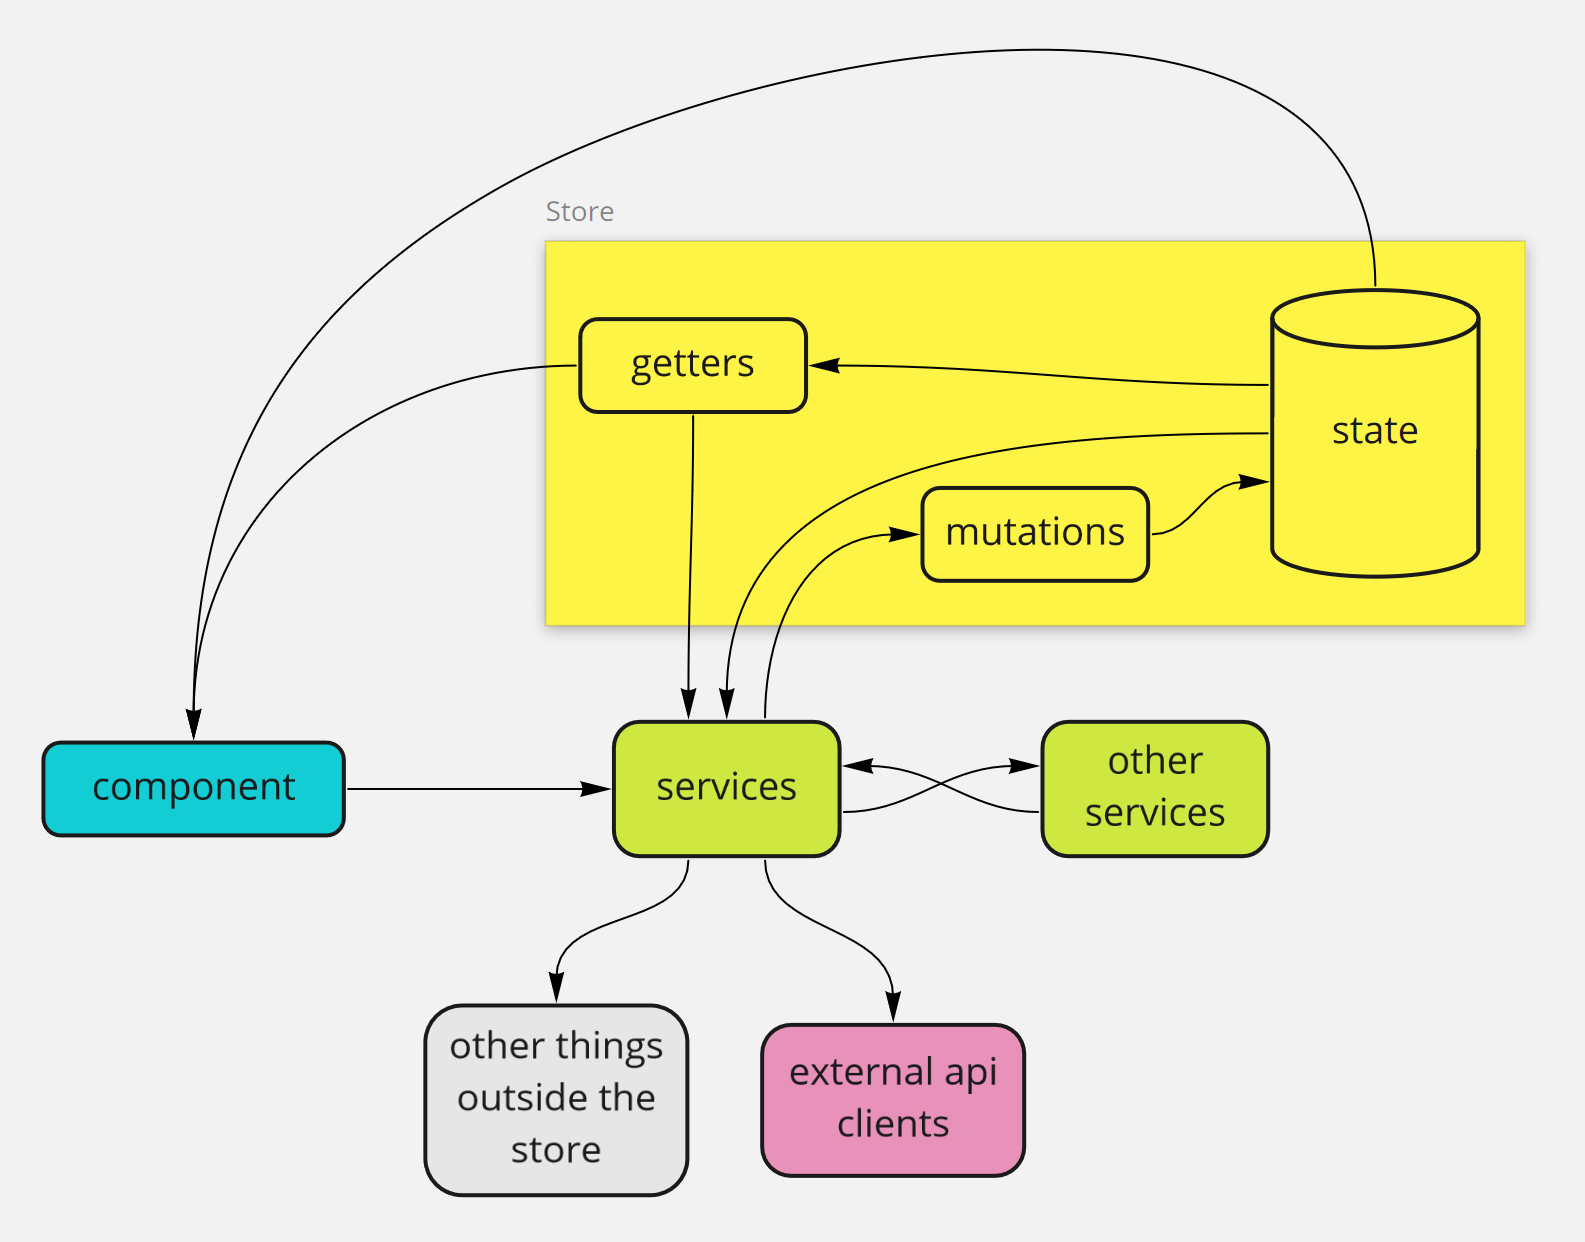
\includegraphics[width=0.7\textwidth]{Images/store.png}
\end{figure}
https://javascript.plainenglish.io/stop-using-actions-in-vuex-a14e23a7b0e6

Finisci di scrivere...

\section{Centralina}
Implementazione centralina


\section{Prodotto Finale}
\label{prodottofinale}
Il prodotto finale ha subito delle evoluzioni rispetto al mockup ma segue le linee
guida imposte.
TODO: Screen di esempio dell'applicazione